\section{Operaciones sobre alfabetos, lenguajes y cadenas}

%Definicion 8
\begin{Def}
La \textit{concatenación} de dos cadenas $w$ e $z$ se denota como $w \cdot z$ ó $wz$ y es la cadena 
que resulta de unir $w$ e $z$. 

\textit{Nota:} La concatenación aplica para \textbf{símbolos}, \textbf{cadenas} y \textbf{lenguajes}.
\end{Def}

\textbf{Ejemplo:}

\begin{itemize}
\item Si $\Sigma = \{0,1\}$, entonces $01$ es una concatenación sobre \textbf{símbolos} de $\Sigma$.
\item Si $w = 01$ e $z = 10$, entonces $wz = w \cdot z = 0110$ es una concatenación sobre \textbf{cadenas}.
\item Si $L_1 = \{0,1\}$ y $L_2 = \{1,0\}$, entonces $L_1L_2 = \{01, 00, 10, 11\}$ es una concatenación sobre \textbf{lenguajes}.
\end{itemize}

%Definicion 9
\begin{Def}
Podemos definir la \textit{potencia} de una cadena $w$ como $w^n = w \cdot w \cdots w$ ($n$ veces), donde $n$ es un número natural. Por ejemplo, si $w = 01$, entonces $w^3 = 010101$.

De manera inductiva tenemos que:

\begin{itemize}
    \item $w^0 = \lambda$ (la cadena vacía)
    \item $w^{n+1} = w^n \cdot w$
\end{itemize}

La potencia la podemos aplicar a \textbf{símbolos}, \textbf{cadenas},\textbf{lenguajes} y \textbf{alfabetos}.
\end{Def}

\textbf{Ejemplo:}

Si $w$ es una \textbf{cadena}, digamos $w = 01$, entonces:

\begin{itemize}
    \item $w^0 = \lambda$
    \item $w^1 = 01$
    \item $w^2 = 0101$
    \item $w^3 = 010101$
\end{itemize}

Si $L$ es un \textbf{lenguaje}, digamos $L = \{00,1\}$, entonces:

\begin{itemize}
    \item $L^0 = \{\lambda\}$
    \item $L^1 = \{00,1\}$
    \item $L^2 = \{(00)00, (00)1, 1(00), (1)1\} = \{0000, 001, 100, 11\}$
\end{itemize}

Para lenguajes $L_1$ y $L_2$, la potencia se define como:

\begin{itemize}
    \item $L_1^0 = \{\lambda\}$
    \item $L_1^1 = L_1$
    \item $L_1^2 = \{xy \mid x \in L_1, y \in L_1\}$
    \item $L_1^3 = \{xyz \mid x \in L_1, y \in L_1, z \in L_1\}$
\end{itemize}

Aquí hay otro ejemplo con $L = \{ab, aab\}$: 
\begin{align*}
    \{ab, aab\}^0 &= \{\epsilon\} \\
    \{ab, aab\}^1 &= \{ab, aab\} \\
    \{ab, aab\}^2 &= \{abab, abaab, aabab, aabaaab\} \\
    \{ab, aab\}^3 &= \{ab(ab)ab, ab(ab)aab, ab(aab)ab, (aab)abab, aab(aab)ab,aab(ab)aab,ab(aab)aab, aab(aab)aab\}
\end{align*}

Como tengo $2$ cadenas y quiero ver todas las combinaciones de $2$ cadenas, entonces tengo $2^2 = 4$ combinaciones. Si quiero ver todas las combinaciones de $3$ cadenas, entonces tengo $2^3 = 8$ combinaciones.
%Definición 10
\begin{Def}
También podemos definir la \textit{potencia} de un alfabeto $\Sigma$ como $\Sigma^n = \{w^n \mid w \in \Sigma^*\}$, donde $\Sigma^*$ es el 
conjunto de todas las cadenas sobre $\Sigma$.
\end{Def}

 Por ejemplo, si $\Sigma = \{0,1\}$, entonces $\Sigma^2 = \{00, 01, 10, 11\}$.

 \begin{align*}
    \Sigma^0 &= \{\lambda\} \\
    \Sigma^1 &= \{0,1\} \\
    \Sigma^2 &= \{00, 01, 10, 11\} \\
    \Sigma^3 &= \{000, 001, 010, 011, 100, 101, 110, 111\} \\
    \vdots \\
    \Sigma^n &= \{w^n \mid w \in \Sigma^*\}
 \end{align*}

 %Definición 11
\begin{Def}
Vamos a definir a la \textit{cerradura de Kleene} o la \textit{estrella de Kleene} de un alfabeto $\Sigma$ como $\Sigma^*$,  
\begin{align*}
    \Sigma^* &= \bigcup_{n \geq 0} \Sigma^n = \Sigma^0 \cup \Sigma^1 \cup \Sigma^2 \cup \ldots \\
    \Sigma^+ &= \Sigma^1 \cup \Sigma^2 \cup \Sigma^3 \cup \ldots \\ 
    \Sigma^* &= \Sigma^+ \cup \{\lambda\}
\end{align*}
Donde $\Sigma^n$ es la potencia del alfabeto. Podemos describir a $\Sigma^*$(sigma estrella) como el conjunto de todas las cadenas (incluida la cadena vacía) 
que se pueden formar a partir de los símbolos de $\Sigma$.
\end{Def}
\textbf{Ejemplo:}

Si $\Sigma = \{0,1\}$, entonces $$\Sigma^* = \{\lambda, 0, 1, 00, 01, 10, 11, 000, 001, 010, 011, 100, 101, 110, 111, \ldots\}$$
es decir, el conjunto de todos los números binarios (incluidos los de longitud cero, a.k.a. la cadena vacía).

%Lema 1
\begin{Lem}
Sea $Q$ un conjunto finito. Entonces, el número de subconjuntos de $Q$ es $2^{|Q|}$, donde $|Q|$ es el número de elementos en $Q$. A este conjunto se le llama \textit{conjunto potencia} de $Q$ y se denota como $\mathcal{P}(Q)$ ó $2^Q$.
\end{Lem}

\textit{Demostración.} Sea $Q$ un conjunto finito con $n$ elementos. Entonces, cada elemento de $Q$ puede estar presente o no en un subconjunto, 
lo que nos da dos opciones (incluir o no incluir) cada elemento. Por lo tanto, el número total de subconjuntos de $Q$ es $2^n = 2^{|Q|}$. \qedsymbol

\newpage
Más adelante cuando veamos autómatas finitos no deterministas, veremos su función de transición, la cual es una función que toma un estado y un símbolo de entrada y devuelve un conjunto de estados. 
Esta función se denota como $\delta: Q \times \{\Sigma \cup \lambda\}\to 2^Q$ (conjunto potencia), donde $Q$ es el conjunto de estados y $\Sigma$ es el alfabeto. 
\begin{figure}
    \centering
    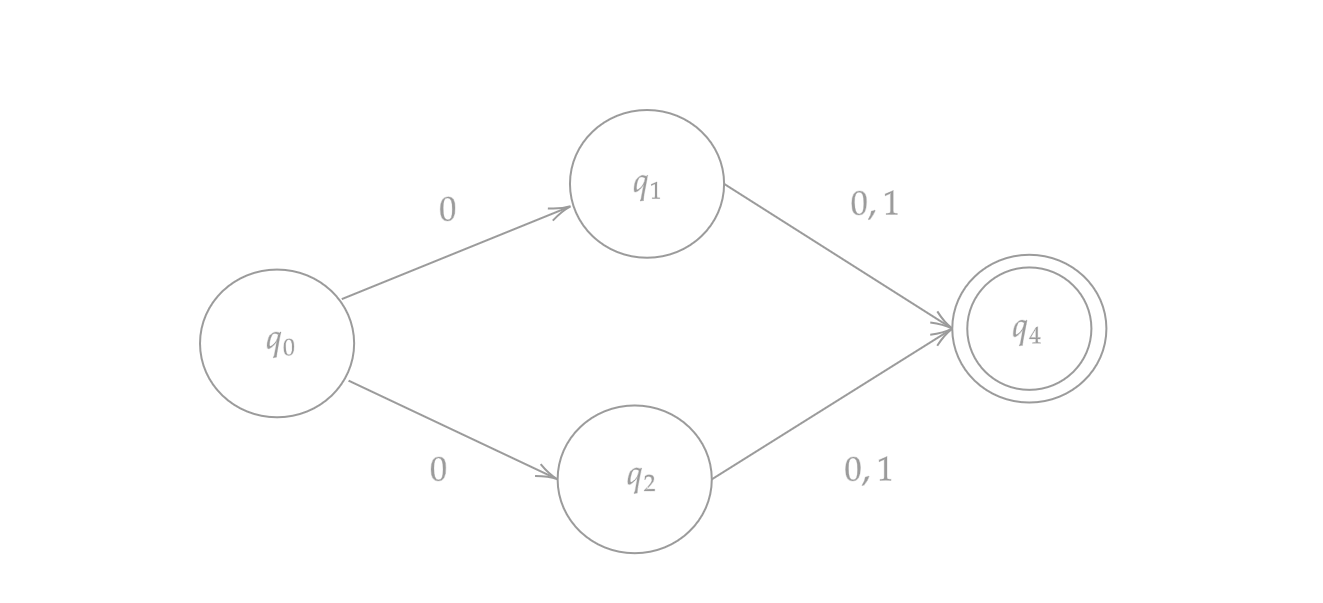
\includegraphics[width=0.7\textwidth]{images/dfa1.png}
    \caption{Ejemplo de un autómata finito determinista (DFA). Este es el autómata que acepta la expresión regular $0(0+1) = \{0, 00, 01\}$.}
\end{figure}

\subsection{Operaciones sobre cadenas}
\begin{Def}
\begin{itemize}
    \item \textbf{Concatenación:} Dadas dos cadenas $x$ e $y$, la concatenación es asociativa: $(x \cdot y) \cdot z = x \cdot (y \cdot z)$ para toda cadena.
    \item La cadena vacía $\lambda$ es la \textbf{identidad} de la concatenación: $x \cdot \lambda = \lambda \cdot x = x$ para toda cadena $x$.
    \item $|x \cdot y| = |x| + |y|$ para toda cadena $x$ e $y$.
    \item $w^m w^n = w^{m+n}$
\end{itemize}
    El conjunto de $(\Sigma^*, \cdot)$ con $\lambda$ como identidad es un monoide, ya que cumple con las propiedades de asociatividad e identidad.
\end{Def}

\subsection{Lenguajes y operaciones sobre lenguajes}


\begin{Def}

Dado un alfabeto $\Sigma$, un \textbf{lenguaje} sobre $\Sigma$ es un subconjunto de $\Sigma^*$. 
Dado un lenguaje $L \subseteq \Sigma^*$, definimos las siguientes operaciones sobre lenguajes:
\begin{itemize}
    \item \textbf{Unión:} $L(a) \cup L(b) = L(a+b)= \{w \mid w \in L_1 \text{ o } w \in L_2\}$
    \item \textbf{Intersección:} $L_1 \cap L_2 = \{w \mid w \in L_1 \text{ y } w \in L_2\}$
    \item \textbf{Concatenación:} $L(a) \cdot L(b) = L(ab) = \{wz \mid w \in L(a), z \in L(b)\}$
    \item \textbf{Diferencia:} $L_1 - L_2 = \{w \mid w \in L_1 \text{ y } w \notin L_2\}$
    \item \textbf{Complemento:} $\overline{L} = \sim L = \{\lambda\} \cup (\Sigma^* - L)$
    \item \textbf{Cerradura de Kleene:} $L^* = \bigcup_{n \geq 0} L^n$
    \item $L^+ = L^* - \{\lambda\} = \bigcup_{n \geq 1} L^n$
\end{itemize}
\end{Def}

Una analogía útil es pensar en los lenguajes es como el el lenguaje español. Sabemos que nuestro
alfabeto es $\Sigma = \{\texttt{a, b, c, \ldots, z}\}$ y que podemos formar palabras (cadenas) con estos símbolos.El 
lenguaje español $L(esp)$ es un subconjunto de $\Sigma^*$. Otro ejemplo es pensar en un lenguaje de programación como $C$, donde el alfabeto es el conjunto de caracteres ASCII y 
el lenguaje es el conjunto de todas las cadenas que son programas válidos en ese lenguaje.
\\ \\ 
Algunos ejemplos de lenguajes son:

\begin{enumerate}
    \item El lenguaje de todas las cadenas que contienen tienen el mismo número de $0$s y $1$s. Para contar el número de caracteres dentro 
    de una cadena podemos usar la notación $\#0(w)$ para el número de $0$s y $\#1(w)$ para el número de $1$s. Entonces, este lenguaje se puede definir como:

    $$L = \{w \in \Sigma^* \mid \#0(w) = \#1(w)\}$$

    \item El lenguaje de todas las cadenas que comienzan con $0$ y terminan con $1$. Este lenguaje se puede definir como:

    $$L = \{w \in \Sigma^* \mid w = 0x1, x \in \Sigma^*\}$$

    \item El lenguaje de todas los números binarios que son primos 
    \begin{align*}
        0  = 0 && \text{No es primo} \\ 
        1  = 1 && \text{No es primo} \\ 
        10 = 2 && \text{Es primo} \\ 
        11 = 3 && \text{Es primo} \\ 
        100 = 4 && \text{No es primo} \\ 
        101 = 5 && \text{Es primo} \\ 
        110 = 6 && \text{No es primo} \\ 
        111 = 7 && \text{Es primo} \\ 
        1000 = 8 && \text{No es primo} \\ 
        1001 = 9 && \text{No es primo} \\ 
        1010 = 10 && \text{No es primo} \\ 
        1011 = 11 && \text{Es primo} \\ 
        1100 = 12 && \text{No es primo} \\ 
        1101 = 13 && \text{Es primo} \\ 
        1110 = 14 && \text{No es primo} \\ 
        1111 = 15 && \text{No es primo} \\ 
    \end{align*}
    $$\{10, 11, 101, 111, 1011, 1101, \dots\}$$

    Seguramente alguna vez hemos programado un verificador de números primos en algún lenguaje de programación. En general, 
    veremos que los lenguajes son conjuntos de cadenas que cumplen ciertas propiedades. Algunos lenguajes son capturados por expresiones regulares o autómatas.

    \subsubsection{Muchas cosas se pueden resolver con lenguajes y autómatas, y muchas cosas que no}

Una de las cosas que resuelven los autómatas es decidir si una cadena pertenece 
o no a un lenguaje. Este es un problema de decisión (Entscheidungsproblem), 
gracias a Turing sabemos que no podemos obtener un sí o no para cualquier problema. 

Un \textit{problema de decisión} puede ser determinar si una cadena $w$ pertenece a un lenguaje $L$. 
Por ejemplo, pensemos en el lenguaje de los números primos, si tenemos cualquier cadena podríamos preguntarnos
si esta representación binaria es un número primo. ¿Dada una cadena $w$, $w \in L_p?$.  

En el siguiente capítulo trataremos las cadenas que sabemos que un autómata sí puede responder. 
Veremos que este autómata tiene limitaciones y más adelante trataremos de rebasarlas con el autómata con pila.
Por ejemplo, el lenguaje $\{0^n1^n \mid n \geq 0\}$ es el conjunto de todas las cadenas que tienen el mismo número de $0$'s seguido del mismo número de $1$'s.
Este lenguaje no puede ser reconocido por un autómata finito, pero si por un autómata con pila. Aunque este último tipo de autómata tiene más potencia, todavía hay lenguajes que no puede reconocer.
Y más adelante veremos que hay lenguajes que no pueden ser reconocidos por ningún autómata, ni siquiera por una máquina de Turing. El quiebre del \href{https://plato.stanford.edu/entries/hilbert-program/}{programa de Hilbert} por querer encontrar
un procedimiento efectivo para decidir si una proposición es verdadera o falsa quedó muerto. 

\begin{figure}
    \centering
    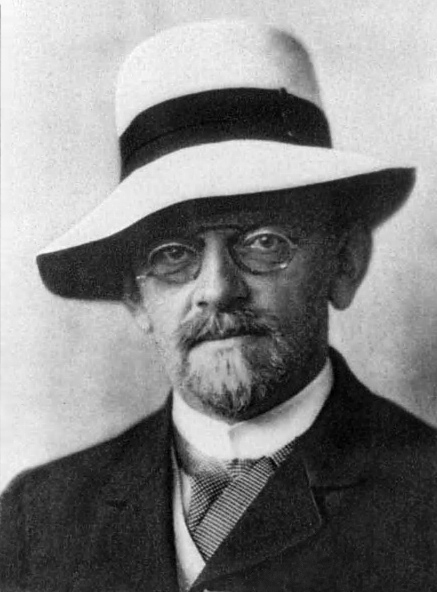
\includegraphics[width=0.4\textwidth]{images/Hilbert.jpg}
    \caption{David Hilbert (1862-1943), un matemático alemán triste.}
\end{figure}

\end{enumerate}

\subsubsection{Operaciones sobre lenguajes}

\textbf{Ejemplo 1}. Sea ($L \in \Sigma^* = \{0,1\}^*$). 

\begin{itemize}
    \item El lenguaje de todas las cadenas que empiezan con $0$ es $L_0 = \{0w \mid w \in \Sigma^*\} = \{0,01,00, 000, 001, \cdots\}$.
    \item El lenguaje de todas las cadenas que terminan con $1$ es $L_1 = \{w1 \mid w \in \Sigma^*\} = \{1, 01, 11, 001, 011, \cdots\}$
\end{itemize}

\begin{itemize}
    \item \textbf{Unión:} $L_1 \cup L_2 = \{0,1,00, 01,11, 000, 001, 010, 011, \cdots\} = \{0w \ \cup \ w1 \mid w \in \Sigma^*\}$
    \item \textbf{Intersección:} $L_1 \cap L_2  = \{ 01, 001, 011, 0001, \cdots\} $
    \item \textbf{Concatenación:} $L_1L_2 = \{01,001,011,101,0101, \cdots\}$ (La concatenación es como un producto cruz de los elementos de ambos lenguajes concatenados)
    \item \textbf{Diferencia:} $L_1 - L_2 = \{0,00,000,001, \cdots\}$
    \item \textbf{Complemento:} $\overline{L_1} = \{1,10,11,100, 101, \cdots\}$
\end{itemize}
 
\textbf{Ejemplo 2}. Sea $L$ el conjunto de letras $\{A,B,C \dots Z, a,b,c, \dots z\}$ y $D$ el conjunto de dígitos $\{0,1, \dots , 9\}$.

\begin{enumerate}
    \item $L \cup D$ es el conjunto de letras y de números, tenemos $62$ símbolos $(26+26+10) = 62$ cadenas de longitud 1. Cada una de estas cadenas es una letra o un dígito. 
    \item $LD$ es el conjunto de $520$ cadenas de longitud 2 $(26 + 26)*2$, cada una siendo una letra concatenada a un número. 
    \item $L^4$ son todas las cadenas con 4 letras. 
    \item $L^*$ son todas las cadenas de letras incluyendo la cadena vacía $\lambda$
    \item $L(L \cup D)^*$ es el conjunto de todas las cadenas de letras y números que empiezan con una letra. 
    \item $D^{+}$ es el conjunto de todas las cadenas de uno o más dígitos.
\end{enumerate}

\subsubsection{Propiedades de las operaciones sobre lenguajes}
\begin{itemize}
    \item \textbf{Conmutatividad de la unión:} $L_1 \cup L_2 = L_2 \cup L_1$
    \item \textbf{Asociatividad de la unión:} $(L_1 \cup L_2) \cup L_3 = L_1 \cup (L_2 \cup L_3)$
    \item \textbf{Conmutatividad de la intersección:} $L_1 \cap L_2 = L_2 \cap L_1$
    \item \textbf{Asociatividad de la intersección:} $(L_1 \cap L_2) \cap L_3 = L_1 \cap (L_2 \cap L_3)$
    \item \textbf{Distributividad de la intersección sobre la unión:} $L_1 \cap (L_2\ \cup L_3) = (L_1 \cap L_2) \cup (L_1 \cap L_3)$
    \item \textbf{Distributividad de la unión sobre la intersección:} $L_1 \cup (L_2 \cap L_3) = (L_1 \cup L_2) \cap (L_1 \cup L_3)$
    \item \textbf{Identidad de la unión:} $L \cup \emptyset = \emptyset \cup L = L$
    \item \textbf{Identidad de la concatenación:} $L \cdot \lambda = \lambda \cdot L = L$
    \item \textbf{El aniquilador:} $L \cdot \emptyset = \emptyset \cdot L = \emptyset$
    \item \textbf{Distributividad de la concatenación(1):} $A(B \cup C) = (AB) \cup (AC)$
    \item \textbf{Distributividad de la concatenación(2):} $(A \cup B)C = (AC) \cup (BC)$
    \item \textbf{Ley de Morgan(1):} $\sim (L_1 \cup L_2) = \sim L_1 \cap \sim L_2$
    \item \textbf{Ley de Morgan(2):} $\sim (L_1 \cap L_2) = \sim L_1 \cup \sim L_2$
    \item \textbf{Propiedades de la cerradura de Kleene(1):} $L^*L^* = L^*$
    \item \textbf{Propiedades de la cerradura de Kleene(2):} $L^{**} = L^*$
    \item \textbf{Propiedades de la cerradura de Kleene(3):} $L^* = \{\lambda\} \cup LL^* = \lambda \cup L^*L$
    \item \textbf{Propiedades de la cerradura de Kleene(4):} $\emptyset^* = \{\lambda\}$
    \item \textbf{Propiedades de la cerradura de Kleene(5):} $L^+ = LL^* = L^*L$
\end{itemize}

    La concatenación no se distribuye sobre la intersección, por ejemplo si $A = \{a,ab\}$, $B = \{b\}$ y $C = \{\epsilon\}$, 
    entonces $A(B \cap C) = \{a,ab\}(\{b\} \cap \{\epsilon\}) = \{a,ab\}{\emptyset} = \emptyset$  pero $(AB) \cap (AC) = \{ab, abb\} \cap \{a, ab\} = ab$. Pero $\emptyset \neq ab$ \textcolor{red}{Contradicción}.